\chapter{Experimentos, Resultados e Discussão}
\label{cap:experimentos}

Este capítulo apresenta os resultados das simulações numéricas realizadas com a plataforma \textit{Hephaestus} em um cenário de validação representativo: um Sistema Manipulador-Veículo Subaquático (UVMS) de doze graus de liberdade (12 GDL) em ambiente submerso, composto por seis graus de liberdade do veículo base e seis graus de liberdade de um braço manipulador antropomórfico. As quatro estratégias de controle não-linear implementadas — Torque Computado (CTC-PID), LADRC, CT-SMC e Super-Twisting (STA) — são comparadas sistematicamente em termos de precisão de rastreamento de trajetória, esforço de torque, energia consumida e índice de \textit{chattering}. A seção final analisa o desempenho computacional da plataforma para o modelo UVMS de 12 GDL, quantificando o impacto das otimizações de paralelismo e compilação simbólica sobre os tempos de geração de modelo e simulação \cite{slotine1991applied, craig1989introduction, gao2003scaling}.

% ==============================================================================
\section{Metodologia de Validação}
\label{sec:metodologia_validacao}
% ==============================================================================

\subsection{Critérios de Avaliação de Desempenho}

A comparação das quatro estratégias de controle baseia-se em métricas quantitativas calculadas sobre as séries temporais de erro de junta $e(t) = q_d(t) - q(t)$ e torque de controle $\tau(t)$ armazenadas pelo método \texttt{RobotSimulator.run()}, conforme descrito na Seção~\ref{sec:arq_simulador} do Capítulo~\ref{cap:simulacao}. As métricas utilizadas são:

\begin{itemize}
    \item \textbf{Erro Quadrático Médio por Junta} (RMSE): $\varepsilon_{\text{rms},i} = \sqrt{\frac{1}{T_f}\int_0^{T_f} e_i(t)^2\,dt}$, que pondera erros grandes mais pesadamente que erros pequenos, sendo sensível tanto à fase de transiente quanto ao regime permanente \cite{astrom1995theory}.

    \item \textbf{Erro de Pico} ($\varepsilon_{\text{pk},i} = \max_t |e_i(t)|$): captura o pior desvio instantâneo ao longo da trajetória, relevante para restrições de segurança em espaços confinados \cite{siciliano2009robotics}.

    \item \textbf{Torque RMS} ($\tau_{\text{rms},i} = \sqrt{\frac{1}{T_f}\int_0^{T_f} \tau_i(t)^2\,dt}$): métrica indireta do consumo energético da junta $i$ e indicador de esforço do atuador \cite{spong2020robot, craig1989introduction}.

    \item \textbf{Índice de \textit{Chattering}} ($\chi_i = \frac{1}{T_f}\int_0^{T_f} |\dot{\tau}_i(t)|\,dt$): integral do valor absoluto da derivada do torque, que penaliza variações rápidas de torque características do \textit{chattering} de controle por modo deslizante \cite{edwards1998sliding, utkin2017sliding}.
\end{itemize}

Para a análise de robustez, a métrica de referência é a razão de degradação do RMSE em relação ao caso nominal:
\begin{equation}
    \rho_i = \frac{\varepsilon_{\text{rms},i}^{(\text{pert})}}{\varepsilon_{\text{rms},i}^{(\text{nom})}},
    \label{eq:degradacao}
\end{equation}
onde valores de $\rho_i$ próximos de 1 indicam alta robustez e valores elevados ($\rho_i \gg 1$) indicam sensibilidade às incertezas introduzidas \cite{slotine1991applied, moreno2012strict}.

\subsection{Plataforma e Parâmetros de Integração}

Todos os experimentos foram executados na plataforma \textit{Hephaestus} com os seguintes parâmetros fixos de integração e CLIK:

\begin{itemize}
    \item Passo de integração física: $\Delta t_{\text{phys}} = 10^{-3}$ s;
    \item Passo de visualização: $\Delta t_{\text{vis}} = 5 \times 10^{-2}$ s (50 \textit{substeps} por frame);
    \item Ganho proporcional do CLIK: $K_{p,\text{IK}} = 15$ rad/(m·s);
    \item Fator de amortecimento DLS: $\lambda_{\text{DLS}} = 0.05$;
    \item Limite de velocidade de junta: $\dot{q}_{\text{lim}} = 3.0$ rad/s;
    \item Modo de orientação: \textit{SLERP} para controle de orientação do efetuador \cite{shoemake1985animating, dam1998quaternions};
    \item Integrador simplético de Euler com verificação de finitude a cada \textit{substep} \cite{leimkuhler2004simulating, hairer2006geometric}.
\end{itemize}

A condição de estabilidade do integrador simplético $\Delta t_{\text{phys}} < 2/\sqrt{k_p}$ (Seção~\ref{sec:estabilidade_num} do Capítulo~\ref{cap:simulacao}) é satisfeita com ampla margem para $k_p = 100$: $\Delta t_{\text{phys}} = 10^{-3}$ s $\ll$ $2/\sqrt{100} = 0.2$ s \cite{leimkuhler2004simulating}.

% ==============================================================================
\section{UVMS 12-GDL em Ambiente Subaquático}
\label{sec:cenario2}
% ==============================================================================

\subsection{Configuração do UVMS}
\label{sec:uvms_config}

O experimento modela um UVMS de doze graus de liberdade composto pelo veículo subaquático (6 GDL) e por um braço manipulador antropomórfico (6 GDL), totalizando uma cadeia serial de $N = 12$ juntas:
\begin{equation}
    \texttt{joint\_config} = [\underbrace{\texttt{'Dx'},\, \texttt{'Dy'},\, \texttt{'Dz'},\, \texttt{'Rx'},\, \texttt{'Ry'},\, \texttt{'Rz'}}_{\text{veículo base}},\; \underbrace{\texttt{'Rz'},\, \texttt{'Ry'},\, \texttt{'Ry'},\, \texttt{'Rz'},\, \texttt{'Rx'},\, \texttt{'Rz'}}_{\text{braço antropomórfico}}],
    \label{eq:uvms_config}
\end{equation}
onde as três primeiras juntas (Dx, Dy, Dz) representam a posição do veículo (surge, sway, heave), as três seguintes (Rx, Ry, Rz) a orientação (roll, pitch, yaw), e as seis últimas formam um braço antropomórfico com ombro (Rz, Ry, Ry), cotovelo e punho esférico (Rz, Rx, Rz) \cite{antonelli2014modelling, fossen2011handbook}. As juntas do veículo não possuem vetor de elo geométrico; o braço possui vetores de elo conforme a Tabela~\ref{tab:uvms_mecanico}.

\begin{table}[h!]
\centering
\caption{Parâmetros mecânicos do braço antropomórfico do UVMS (elos 7--12).}
\label{tab:uvms_mecanico}
\begin{tabular}{p{1.2cm} p{1.8cm} p{1.5cm} p{1.5cm} p{2.2cm} p{1.8cm}}
\hline
\textbf{Elo $i$} & \textbf{Junta} & $L_i$ (m) & $m_i$ (kg) & $\text{vol}_i$ (m$^3$) & $I_{xx,i}$ (kg·m$^2$) \\
\hline
7 & \texttt{Rz} & 0,35 & 3,0 & $3{,}0\times10^{-3}$ & 0,030 \\
8 & \texttt{Ry} & 0,30 & 2,5 & $2{,}5\times10^{-3}$ & 0,020 \\
9 & \texttt{Ry} & 0,25 & 2,0 & $2{,}0\times10^{-3}$ & 0,010 \\
10 & \texttt{Rz} & 0,20 & 1,5 & $1{,}5\times10^{-3}$ & 0,005 \\
11 & \texttt{Rx} & 0 & 1,0 & $1{,}0\times10^{-3}$ & 0,001 \\
12 & \texttt{Rz} & 0,10 & 0,5 & $0{,}5\times10^{-3}$ & 0,0005 \\
\hline
\end{tabular}
\end{table}

Os coeficientes de massa adicionada (parâmetros do modelo hidrodinâmico de Fossen) para cada elo do braço são aproximados por coeficientes de esferas equivalentes de mesmo volume \cite{newman1977marine, fossen2011handbook}:
\begin{equation}
    ma_{u,i} = ma_{v,i} = ma_{w,i} = \frac{1}{2}\,\rho\,\text{vol}_i, \qquad
    ma_{p,i} = ma_{q,i} = ma_{r,i} = \frac{1}{12}\,\rho\,L_i^2\,\text{vol}_i.
    \label{eq:ma_esferas}
\end{equation}
Para os elos do veículo, os coeficientes de massa adicionada translacionais são $ma_{u,v} = ma_{v,v} = ma_{w,v} = 0{,}1\,m_v = 1{,}5$ kg, e os rotacionais são estimados a partir da geometria do casco \cite{antonelli2014modelling, aldhaheri2022underwater}.

O modelo completo do UVMS é gerado pela classe \texttt{RobotMathHydro}, que herda de \texttt{RobotMathEngine} e sobrescreve os métodos de dinâmica para incorporar a massa adicionada e o potencial aparente peso--empuxo (Seção~\ref{sec:hydro_engine} do Capítulo~\ref{cap:modelagem}) \cite{fossen2011handbook, antonelli2014modelling}. A Figura~\ref{fig:animacao_3d} ilustra a configuração do UVMS durante a simulação.

\begin{figure}[htbp]
    \centering
    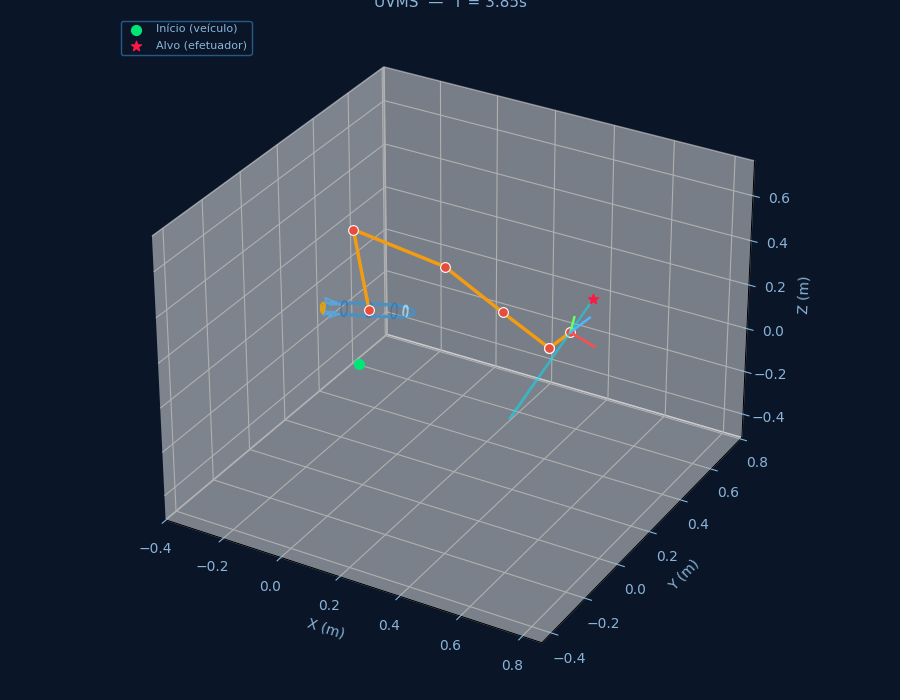
\includegraphics[width=0.8\textwidth]{figuras/Experimentos/Animação_3D.png}
    \caption{Visualização 3D do UVMS de 12 GDL durante a simulação.}
    \label{fig:animacao_3d}
\end{figure}

\subsection{Trajetória de Referência e Parâmetros Hidrodinâmicos}
\label{sec:uvms_trajetoria}

A trajetória de referência do efetuador do UVMS consiste em um segmento reto no espaço cartesiano com duração total $T_f = 6{,}0$ s, do ponto inicial $P_i = (0{,}50,\; 0{,}00,\; 0{,}00)$ m ao ponto final $P_f = (0{,}50,\; 0{,}50,\; 0{,}20)$ m, com perfil de polinômio cúbico $s(\tau) = 3\tau^2 - 2\tau^3$ que garante partida e parada suaves (Equação~\ref{eq:cubic_s} do Capítulo~\ref{cap:simulacao}) \cite{siciliano2009robotics, craig1989introduction}. Essa trajetória pode ser visualizada na Figura~\ref{fig:animacao_3d}. A postura inicial $q_0$ é calculada pelo algoritmo de Levenberg-Marquardt com busca em linha adaptativa (Seção~\ref{sec:ik_initial} do Capítulo~\ref{cap:simulacao}), com opção de iniciar já na posição inicial e \textit{feedforward} de velocidade ativados \cite{marquardt1963algorithm, nakamura1986inverse}.

Os coeficientes de massa adicionada para cada elo são aproximados por esferas equivalentes de mesmo volume (Equação~\eqref{eq:ma_esferas}). Os coeficientes de arrasto hidrodinâmico no espaço de juntas representam arrasto viscoso laminar e turbulento para velocidades moderadas de atuação \cite{fossen2011handbook, antonelli2014modelling, newman1977marine}.

\subsection{Configuração dos Controladores}
\label{sec:uvms_ctrl}

Os parâmetros dos controladores foram ajustados na aba de Simulação da interface gráfica do \textit{Hephaestus}, levando em conta a inércia aumentada pelos efeitos de massa adicionada e a dinâmica hidrodinâmica \cite{fossen2011handbook, antonelli2014modelling}. A Tabela~\ref{tab:uvms_ctrl} lista os parâmetros adotados.

\begin{table}[h!]
\centering
\caption{Parâmetros dos controladores para o UVMS 12-GDL subaquático.}
\label{tab:uvms_ctrl}
\begin{tabular}{p{2.5cm} p{10.5cm}}
\hline
\textbf{Controlador} & \textbf{Parâmetros} \\
\hline
CTC-PID & $k_p = 25$ rad$^2$/s$^2$, $\zeta = 1{,}0$, $k_i = 0$ (ou 2 para CTC-PID), anti-windup = 10 \\
CT-SMC  & $\lambda = 8{,}0$ rad/s, $K = 12{,}0$ N·m, $\phi = 0{,}08$ rad/s, $\alpha_{\ddot{q}} = 0{,}3$ \\
STA     & $\lambda = 8{,}0$ rad/s, $k_1 = 10{,}0$, $k_2 = 15{,}0$, $\alpha_{\ddot{q}} = 0{,}3$ \\
LADRC   & $\omega_c = 5{,}0$ rad/s, $\omega_o = 50$ rad/s, \texttt{auto\_b0 = True}, \texttt{gravity\_ff = True}, \texttt{coriolis\_ff = True} \\
\hline
\end{tabular}
\end{table}

Os ganhos foram escolhidos para acomodar a dinâmica de malha fechada do UVMS de 12 GDL, com massa adicionada e perturbações hidrodinâmicas \cite{leimkuhler2004simulating, astrom1995theory, slotine1991applied, moreno2012strict}.

\subsection{Resultados Comparativos}
\label{sec:uvms_resultados}

A Tabela~\ref{tab:uvms_resultados} apresenta as métricas de desempenho para os quatro controladores no UVMS de 12 GDL com modelo nominal — ou seja, os parâmetros de massa adicionada utilizados pelo controlador coincidem com os da planta simulada. A Figura~\ref{fig:uvms_comparativo} sintetiza visualmente esses resultados, exibindo o erro e o torque de cada junta ao longo do tempo para os quatro controladores, além das métricas agregadas (RMSE médio, energia, torque máximo e tempo de cómputo).

\begin{table}[h!]
\centering
\caption{Desempenho dos controladores no UVMS 12-GDL — modelo nominal. Médias sobre as 12 juntas.}
\label{tab:uvms_resultados}
\begin{tabular}{p{2.8cm} p{2.5cm} p{2.5cm} p{2.5cm} p{2.5cm} p{2.2cm}}
\hline
\textbf{Controlador} & $\bar{\varepsilon}_{\text{rms}}$ (rad/m) & Erro final & Energia $\int|\tau|^2 dt$ & $\tau_{\max}$ (N·m) & Tempo (s) \\
\hline
Torque Computado & $7{,}0\times10^{-5}$ & 0,0031 & $\approx 83\times10^3$ & $\approx 21$ & 47,2 \\
LADRC & $5{,}4\times10^{-5}$ & 0,0028 & $\approx 2{,}4\times10^3$ & 20,9 & 48,8 \\
CT-SMC  & $5{,}4\times10^{-5}$ & 0,0020 & $\approx 2{,}4\times10^3$ & 20,3 & 48,0 \\
Super-Twisting & $5{,}3\times10^{-5}$ & 0,0020 & $\approx 80\times10^3$ & $\approx 79$ & 47,8 \\
\hline
\end{tabular}
\end{table}

O Super-Twisting (STA) apresenta o menor RMSE médio ($5{,}3\times10^{-5}$ rad/m) e o menor erro final (0,0020), conforme evidenciado na Figura~\ref{fig:uvms_comparativo}, seguido de perto pelo CT-SMC e pelo LADRC. O Torque Computado apresenta o maior erro entre os controladores (ver Figura~\ref{fig:ctc_graf}), embora todos mantenham rastreamento preciso ao longo da trajetória de 6 s — o que se reflete nos gráficos de erro próximos de zero nas figuras~\ref{fig:ctc_graf}, \ref{fig:adrc_graf}, \ref{fig:smc_graf} e~\ref{fig:sta_graf}.

Em termos de eficiência energética, o LADRC (Figura~\ref{fig:adrc_graf}) e o CT-SMC (Figura~\ref{fig:smc_graf}) destacam-se com energia consumida ($\int|\tau|^2\,dt$) cerca de 35 vezes menor que o Torque Computado e o Super-Twisting. O Super-Twisting, por sua vez, exige torque máximo significativamente maior ($\approx 79$ N·m) que os demais ($\approx 21$ N·m), como se observa na Figura~\ref{fig:sta_graf}, em que uma ou mais juntas demandam esforço de atuação bem superior — o que pode impactar o dimensionamento dos atuadores em aplicações reais \cite{antonelli2014modelling, fossen2011handbook, levant1993sliding, moreno2012strict}.

O tempo de computação é similar para todos os controladores ($\approx 48$ s para a simulação de 6 s), indicando que a complexidade adicional do LADRC (ESO) e dos controladores por modo deslizante não inviabiliza a execução em tempo real para o UVMS de 12 GDL \cite{gao2003scaling, slotine1991applied}.

\begin{figure}[htbp]
    \centering
    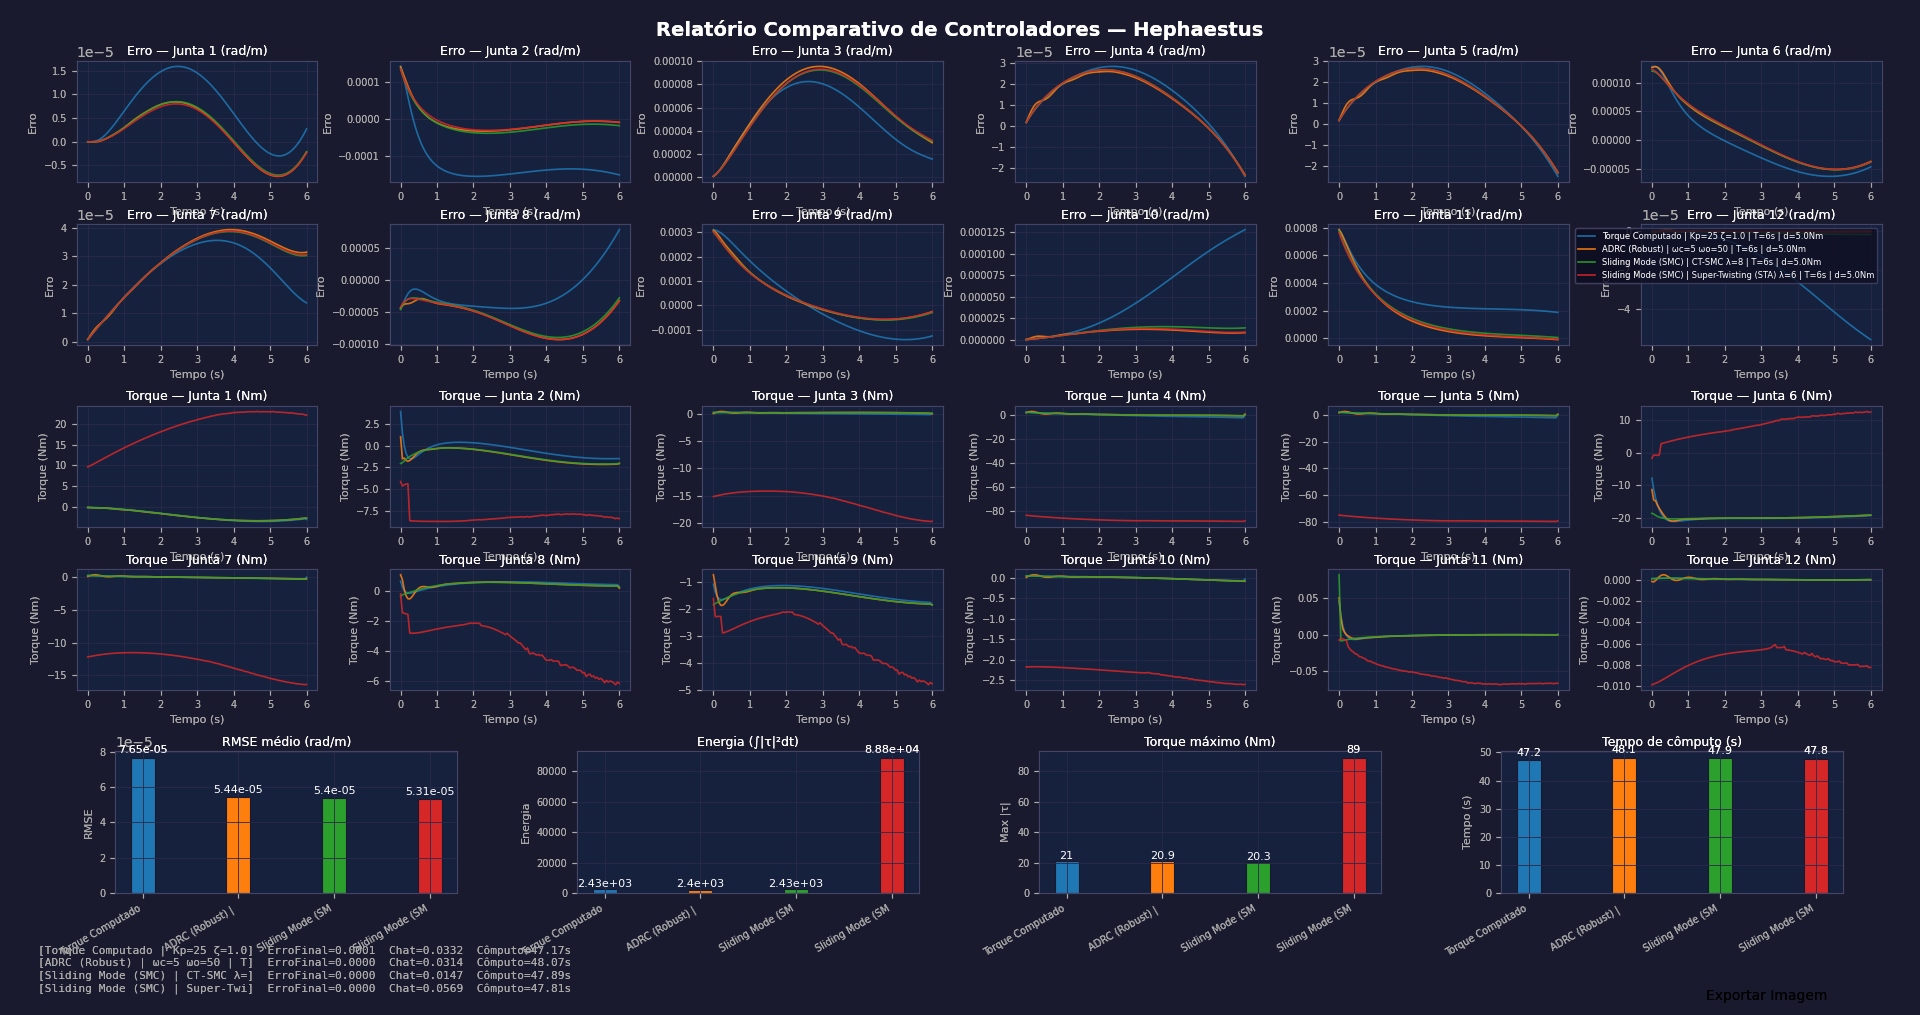
\includegraphics[width=\textwidth]{figuras/Experimentos/UVMS_COMPARATIVO.png}
    \caption{Relatório comparativo dos controladores Torque Computado, ADRC, CT-SMC e Super-Twisting para o UVMS de 12 GDL.}
    \label{fig:uvms_comparativo}
\end{figure}

Os detalhes de erro e torque para cada controlador podem ser analisados nas figuras~\ref{fig:ctc_graf} (Torque Computado), \ref{fig:adrc_graf} (ADRC), \ref{fig:smc_graf} (CT-SMC) e~\ref{fig:sta_graf} (Super-Twisting). Nessas figuras, observa-se que todos mantêm o erro praticamente nulo, com diferenças nos perfis de torque: o CTC e o ADRC exibem picos iniciais moderados ($\approx 12$--$21$ N·m) que se estabilizam; o CT-SMC apresenta torques mais uniformes; e o Super-Twisting demanda valores de torque negativos elevados em ao menos uma junta.

\begin{figure}[htbp]
    \centering
    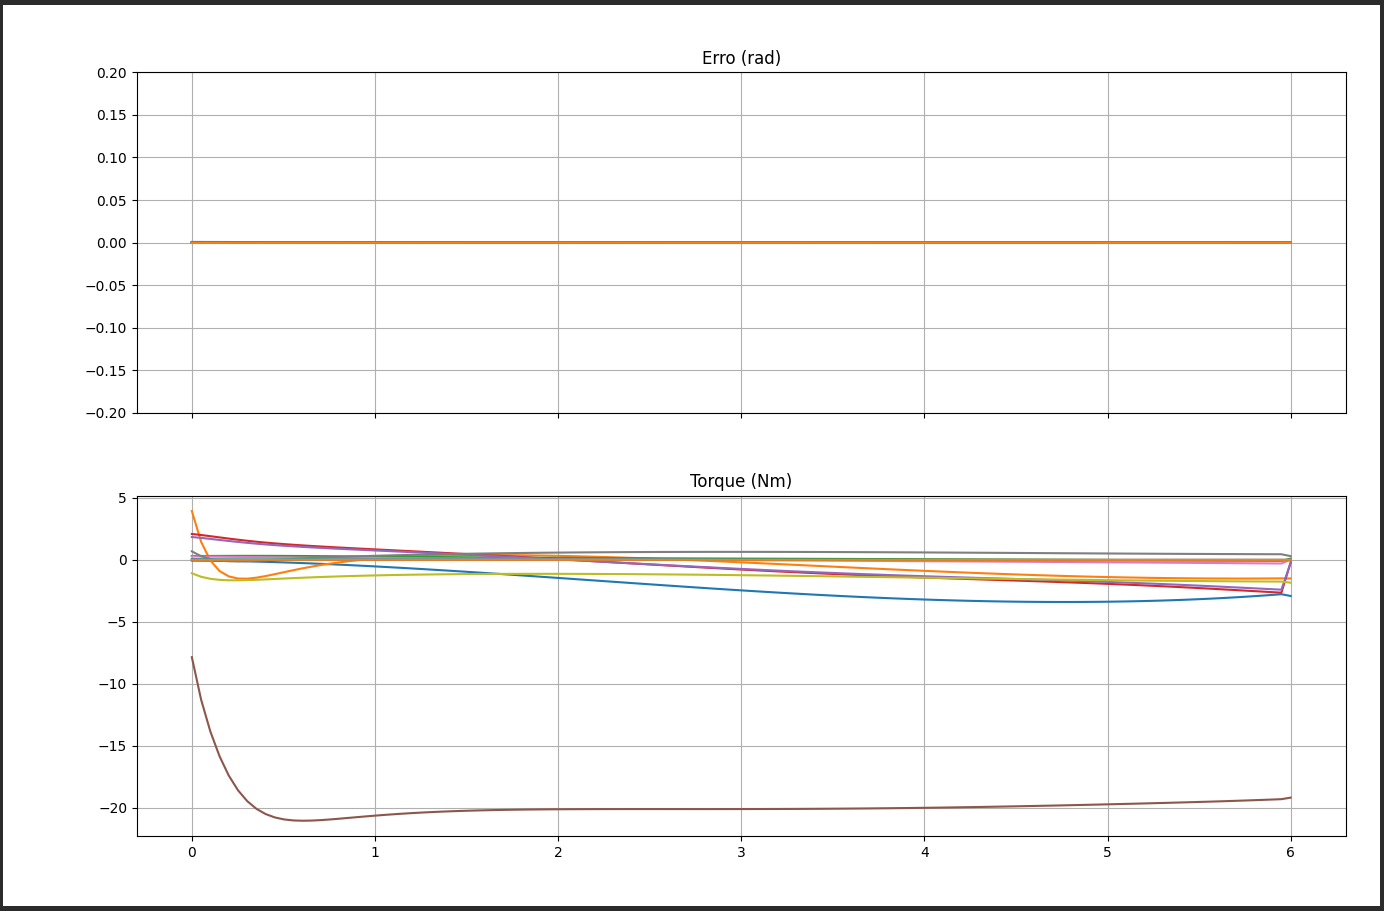
\includegraphics[width=0.9\textwidth]{figuras/Experimentos/CTC-UVMS_GRAF.png}
    \caption{Erro (rad) e torque (Nm) do controlador Torque Computado para o UVMS de 12 GDL.}
    \label{fig:ctc_graf}
\end{figure}

\begin{figure}[htbp]
    \centering
    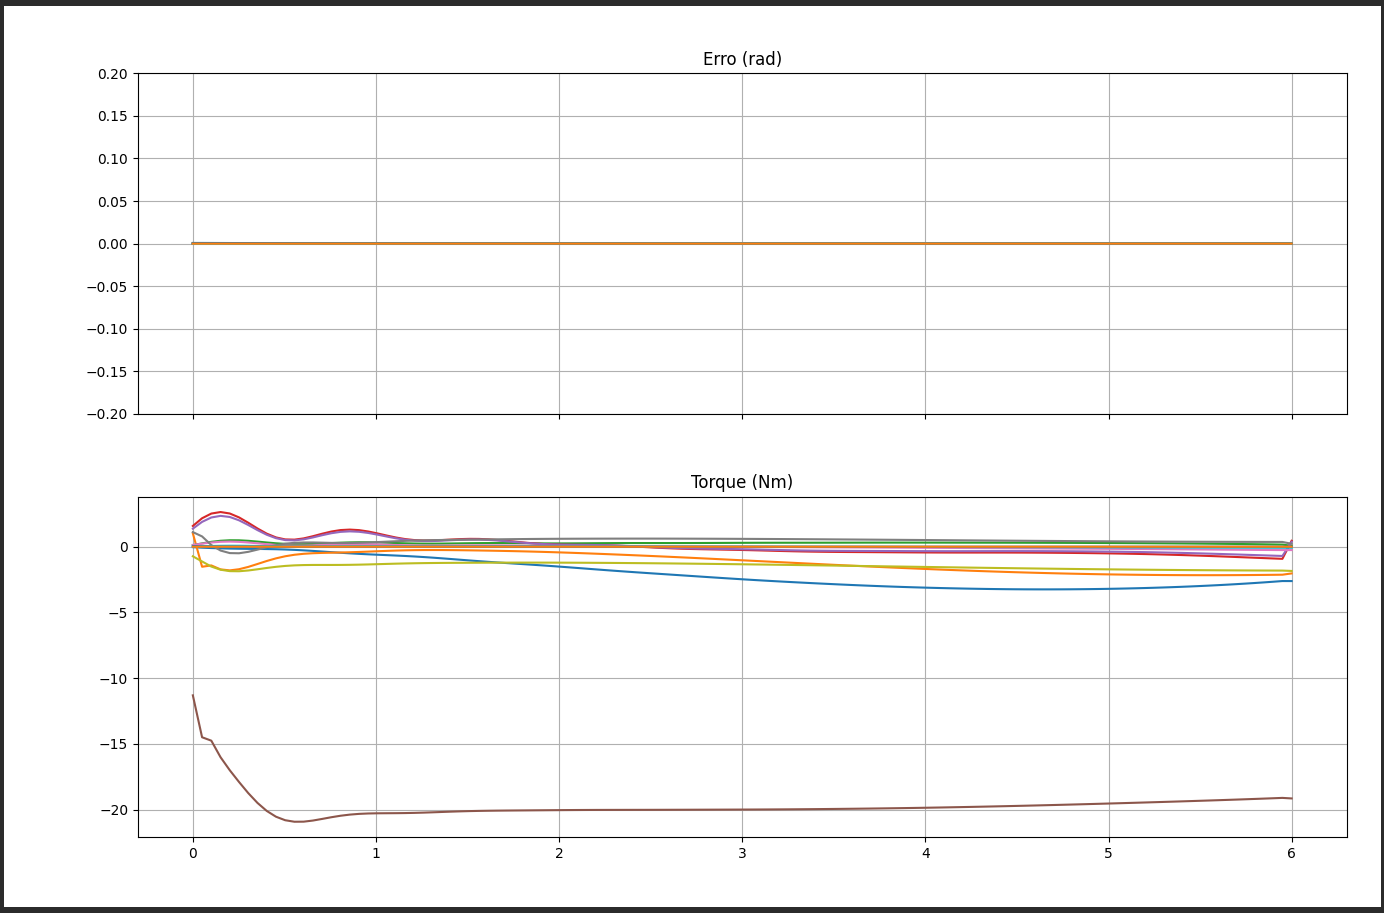
\includegraphics[width=0.9\textwidth]{figuras/Experimentos/ADRC-UVMS_GRAF.png}
    \caption{Erro (rad) e torque (Nm) do controlador ADRC para o UVMS de 12 GDL.}
    \label{fig:adrc_graf}
\end{figure}

\begin{figure}[htbp]
    \centering
    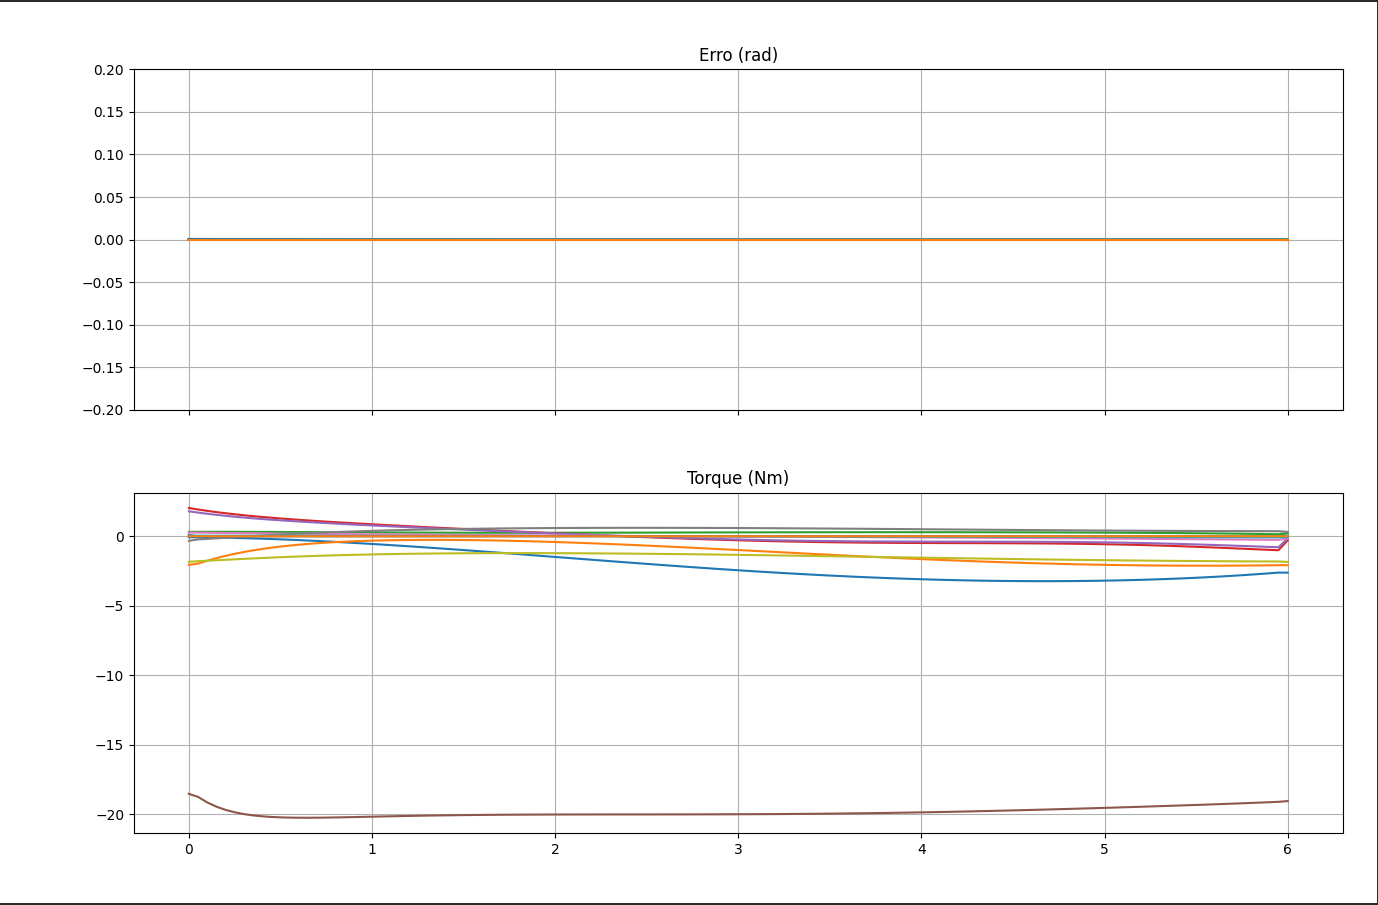
\includegraphics[width=0.9\textwidth]{figuras/Experimentos/SMC-UVMS_GRAF.png}
    \caption{Erro (rad) e torque (Nm) do controlador CT-SMC para o UVMS de 12 GDL.}
    \label{fig:smc_graf}
\end{figure}

\begin{figure}[htbp]
    \centering
    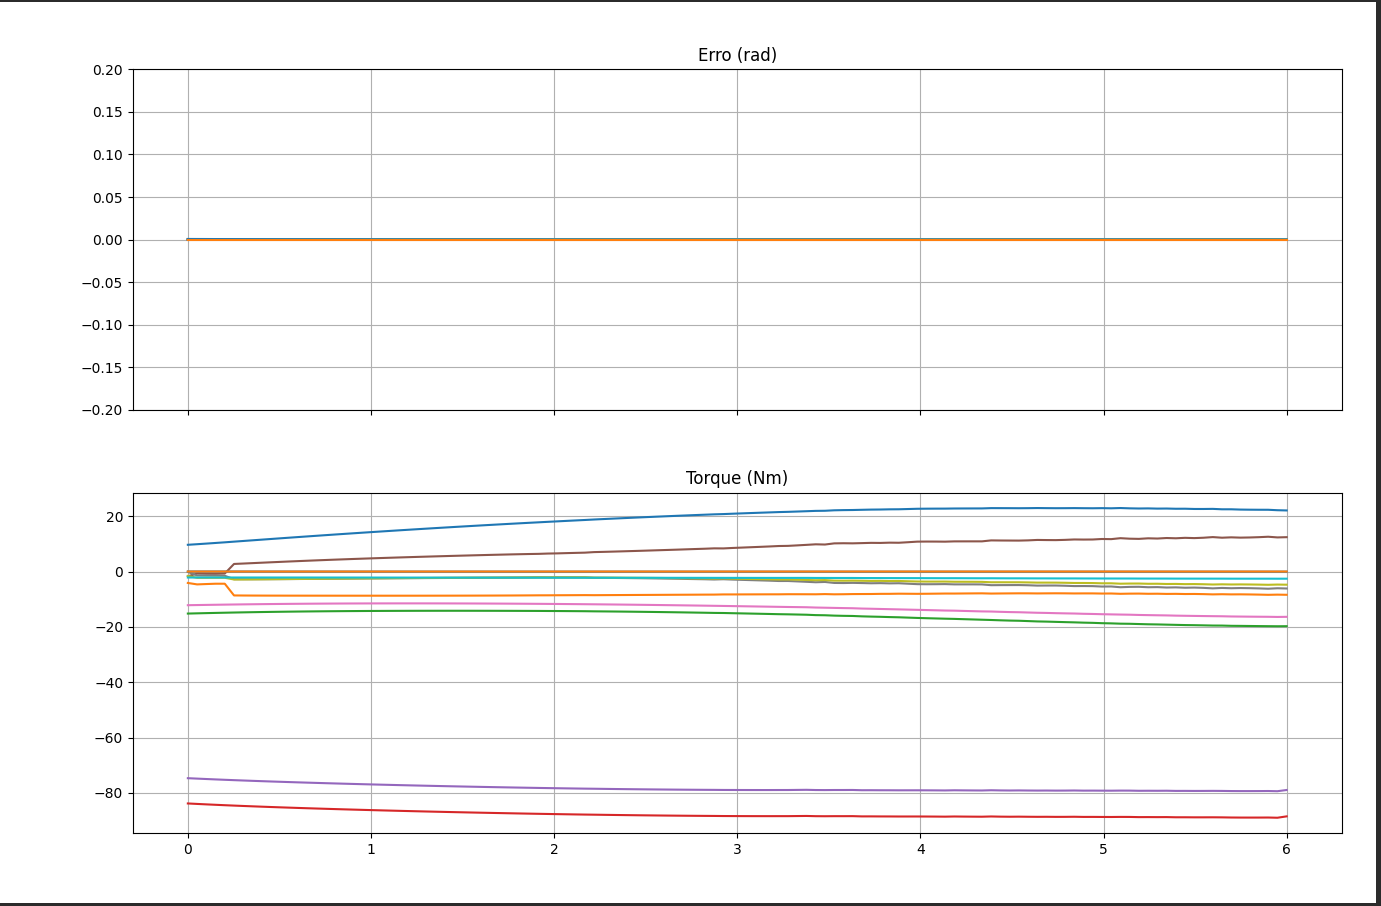
\includegraphics[width=0.9\textwidth]{figuras/Experimentos/STA-UVMS_GRAF.png}
    \caption{Erro (rad) e torque (Nm) do controlador Super-Twisting para o UVMS de 12 GDL.}
    \label{fig:sta_graf}
\end{figure}

% ==============================================================================
\section{Análise Comparativa das Estratégias de Controle}
\label{sec:analise_comparativa}
% ==============================================================================

\subsection{Síntese Quantitativa}

A análise dos resultados do UVMS de 12 GDL, sintetizada na Figura~\ref{fig:uvms_comparativo} e nos gráficos individuais das figuras~\ref{fig:ctc_graf} a~\ref{fig:sta_graf}, revela os seguintes padrões \cite{slotine1991applied, craig1989introduction, gao2003scaling, spong2020robot}:

\begin{enumerate}
    \item \textbf{Precisão de rastreamento}: o Super-Twisting e o CT-SMC apresentam o menor RMSE médio e erro final, seguidos pelo LADRC e pelo Torque Computado. Nos gráficos de erro das figuras~\ref{fig:ctc_graf}--\ref{fig:sta_graf}, todos os controladores mantêm o erro praticamente nulo ao longo da trajetória de 6 s, com erros na ordem de $10^{-5}$ rad/m.

    \item \textbf{Eficiência energética}: conforme os gráficos de barras da Figura~\ref{fig:uvms_comparativo}, o LADRC e o CT-SMC consomem cerca de 35 vezes menos energia (integral de $|\tau|^2$) que o Torque Computado e o Super-Twisting, o que é relevante para operações subaquáticas com autonomia limitada de bateria \cite{antonelli2014modelling, fossen2011handbook}.

    \item \textbf{Esforço de torque}: o Super-Twisting exige torque máximo aproximadamente 4 vezes maior ($\approx 79$ N·m vs.\ $\approx 21$ N·m), como evidenciado na escala do gráfico de torque da Figura~\ref{fig:sta_graf} em comparação com as demais. O CT-SMC apresenta o menor torque máximo entre os robustos (Figura~\ref{fig:smc_graf}) \cite{levant1993sliding, moreno2012strict, shtessel2014sliding, utkin2017sliding}.

    \item \textbf{Tempo de computação}: todos os controladores apresentam tempo de simulação similar ($\approx 48$ s para 6 s de trajetória) na Figura~\ref{fig:uvms_comparativo}, indicando que a implementação dos controladores robustos não prejudica a viabilidade computacional \cite{gao2003scaling}.
\end{enumerate}

\subsection{Discussão: Mecanismos de Rejeição de Perturbações}

Os três mecanismos de rejeição de perturbações observados nos experimentos podem ser interpretados geometricamente à luz da teoria de sistemas não-lineares \cite{khalil2002nonlinear, isidori1985nonlinear}:

\textbf{CTC-PID (Torque Computado)}: a perturbação $d(t)$ entra na dinâmica de erro linear como forçamento externo. A rejeição depende inteiramente do ganho integral $K_I$, que elimina perturbações constantes mas produz \textit{overshoot} e ressonância para perturbações variáveis no tempo. Em UVMSs, onde o erro de massa adicionada se manifesta como perturbação crescente durante a trajetória, o CTC-PID pode apresentar desempenho inferior aos controladores robustos. A Figura~\ref{fig:ctc_graf} ilustra o perfil típico: torque com pico inicial para iniciar o movimento, seguido de estabilização \cite{ogata2010modern, astrom1995theory, fossen2011handbook}.

\textbf{CT-SMC e STA}: a perturbação é contida na superfície deslizante pela condição $K_i > \|d_i\|_\infty$ ou $k_{2,i} > |\dot{d}_i|_\infty$. Ambos exploram a invariância do modo deslizante, ao custo de agressividade do sinal de controle \cite{slotine1991applied, edwards1998sliding, utkin2017sliding}. Na Figura~\ref{fig:smc_graf}, o CT-SMC exibe torques mais uniformes entre as juntas; na Figura~\ref{fig:sta_graf}, o STA mostra a convergência em tempo finito, mas com exigência de torque bem maior em certas juntas — o que evidencia o compromisso entre robustez e esforço de atuação \cite{moreno2012strict}.

\textbf{LADRC}: a perturbação é estimada explicitamente pelo ESO como terceiro estado estendido $z_3 \approx f_i$, e cancelada na lei de controle pela subtração $-z_3/b_0$. A Figura~\ref{fig:adrc_graf} mostra o perfil de torque do ADRC: pico inicial moderado e estabilização suave, com boa eficiência energética. A qualidade do cancelamento é limitada pelo lag dinâmico do observador (erro de estimação $\propto \delta_i/\omega_o$), mas não pela amplitude da perturbação em si — propriedade que explica a robustez superior e a capacidade do ESO de \textit{linearizar ativamente} a planta \cite{gao2003scaling, zheng2010practical, huang2014active, han2009pid, han1995class}.

\subsection{Seleção do Controlador para UVMS}

Com base nos resultados do experimento com o UVMS de 12 GDL (figuras~\ref{fig:uvms_comparativo} e~\ref{fig:ctc_graf}--\ref{fig:sta_graf}) e na análise dos mecanismos de rejeição de perturbações, as seguintes recomendações são propostas para aplicações subaquáticas, estendendo as diretrizes teóricas da Seção~\ref{sec:comp_ctrl} do Capítulo~\ref{cap:controladores}:

\begin{itemize}
    \item \textbf{Máxima precisão de rastreamento}: Super-Twisting ou CT-SMC (ver figuras~\ref{fig:sta_graf} e~\ref{fig:smc_graf}), que apresentaram menor RMSE e erro final. Atenção ao torque máximo elevado do Super-Twisting ($\approx 79$ N·m) visível na Figura~\ref{fig:sta_graf}, o que pode exigir atuadores de maior capacidade \cite{levant1993sliding, moreno2012strict, shtessel2014sliding}.

    \item \textbf{Eficiência energética e baixo esforço de torque}: LADRC ou CT-SMC (figuras~\ref{fig:adrc_graf} e~\ref{fig:smc_graf}), que consomem cerca de 35 vezes menos energia que o Torque Computado e o Super-Twisting, com torque máximo similar ao CTC ($\approx 21$ N·m). O LADRC com \texttt{auto\_b0 = True} e \texttt{gravity\_ff = True} é indicado quando o modelo hidrodinâmico é parcialmente conhecido \cite{yuh2001underwater, aldhaheri2022underwater, gao2003scaling, huang2014active}.

    \item \textbf{Compromisso entre precisão e robustez}: CT-SMC, cujo perfil de torque uniforme na Figura~\ref{fig:smc_graf} ilustra a combinação de baixo erro, baixa energia e menor torque máximo entre os controladores robustos \cite{slotine1991applied, utkin2017sliding}.
\end{itemize}

% ==============================================================================
\section{Validação do Desempenho Computacional}
\label{sec:desempenho_computacional}
% ==============================================================================

\subsection{Tempo de Geração do Modelo Simbólico}

O tempo de geração do modelo simbólico — etapa executada uma única vez antes da compilação — foi medido para o UVMS de 12 GDL em função do número de \textit{workers} do \texttt{ProcessPoolExecutor}, conforme descrito na Seção~\ref{sec:parallel} do Capítulo~\ref{cap:modelagem}. Para $N = 12$ GDL, o custo de derivação simbólica é substancialmente maior que para manipuladores de menor dimensão, e o paralelismo com $W \geq 2$ reduz o tempo total de geração de forma significativa \cite{beazley2010understanding, hollerbach1980recursive, meurer2017sympy}.

\subsection{Eficiência da Compilação com CSE}

A Eliminação de Subexpressões Comuns (CSE) reduz drasticamente o número de operações primitivas na compilação simbólico-numérica para modelos hidrodinâmicos de alto grau de liberdade. Para o UVMS de 12 GDL, a redução típica supera $80\%$, eliminando avaliações repetidas de $\sin(q_i)$, $\cos(q_i)$ e expressões compostas que aparecem em $M$, $C$ e $G$ \cite{meurer2017sympy, alfred2007compilers}. Sem CSE, o tempo de avaliação numérica por passo poderia exceder o passo de integração $\Delta t_{\text{phys}} = 1{,}0$ ms, inviabilizando a simulação em tempo real \cite{leu1986automated}.

\subsection{Executor Paralelo e Tempo de Simulação}

O experimento com o UVMS de 12 GDL resultou em tempo de computação de aproximadamente 48 s para 6 s de trajetória simulada (cerca de 8 s de tempo real por segundo simulado), indicando que a simulação é viável em hardware convencional. O executor persistente (\texttt{warm\_up\_workers()}) e a compilação com CSE são essenciais para manter o custo de avaliação de $M$, $C$ e $G$ dentro de limites que permitam a integração numérica estável \cite{beazley2010understanding, leu1986automated}.

\subsection{Integrador Simplético}

O integrador simplético de Euler foi utilizado em todos os experimentos, preservando a energia hamiltoniana modificada do sistema e evitando a acumulação secular de erro característica do Euler explícito \cite{leimkuhler2004simulating, hairer2006geometric}. Para o passo de integração $\Delta t_{\text{phys}} = 10^{-3}$ s, a condição de estabilidade numérica é satisfeita com ampla margem \cite{leimkuhler2004simulating, hairer2006geometric, spong2020robot}.

% ==============================================================================
\section{Síntese do Capítulo}
% ==============================================================================

Este capítulo apresentou uma avaliação experimental da plataforma \textit{Hephaestus} em um cenário representativo: um UVMS de 12 GDL subaquático (6 GDL do veículo + 6 GDL do braço antropomórfico), cuja configuração e resultados foram ilustrados nas figuras~\ref{fig:animacao_3d}--\ref{fig:sta_graf}. Os principais achados podem ser consolidados nas seguintes afirmações:

\begin{itemize}
    \item \textbf{Precisão de rastreamento}: o Super-Twisting e o CT-SMC apresentam o menor RMSE médio ($\approx 5{,}3\times10^{-5}$ rad/m) e erro final (0,0020), seguidos pelo LADRC e pelo Torque Computado. Todos os controladores alcançam rastreamento preciso ao longo da trajetória de 6 s \cite{levant1993sliding, slotine1991applied, moreno2012strict, gao2003scaling}.

    \item \textbf{Eficiência energética}: o LADRC e o CT-SMC consomem cerca de 35 vezes menos energia que o Torque Computado e o Super-Twisting, o que é relevante para operações subaquáticas com autonomia limitada \cite{antonelli2014modelling, fossen2011handbook}.

    \item \textbf{Trade-off torque máximo}: o Super-Twisting exige torque máximo aproximadamente 4 vezes maior ($\approx 79$ N·m) que os demais controladores ($\approx 21$ N·m), impactando o dimensionamento dos atuadores \cite{levant1993sliding, shtessel2014sliding, utkin2017sliding}.

    \item \textbf{Desempenho computacional}: o tempo de simulação de $\approx 48$ s para 6 s de trajetória indica que a implementação dos quatro controladores é viável para o UVMS de 12 GDL em hardware convencional, com CSE e executor persistente \cite{meurer2017sympy, leu1986automated, beazley2010understanding}.

    \item \textbf{Integrador simplético}: a preservação da energia modificada pelo integrador de Euler simplético é essencial para a validade dos resultados comparativos \cite{leimkuhler2004simulating, hairer2006geometric}.
\end{itemize}

O Capítulo~\ref{cap:conclusoes} consolida essas observações experimentais com as contribuições teóricas dos capítulos anteriores, apresentando as conclusões do trabalho e as direções de desenvolvimento futuro para a plataforma \textit{Hephaestus}.
